% Generated by julia/scripts/generate_manuscript_numerical_artifacts.jl.
% Sources: registered financial mechanism, decomposition, grammar, candidate-audit,
% and annual episode-ranking CSVs. The locked scoring engines are not rerun here.
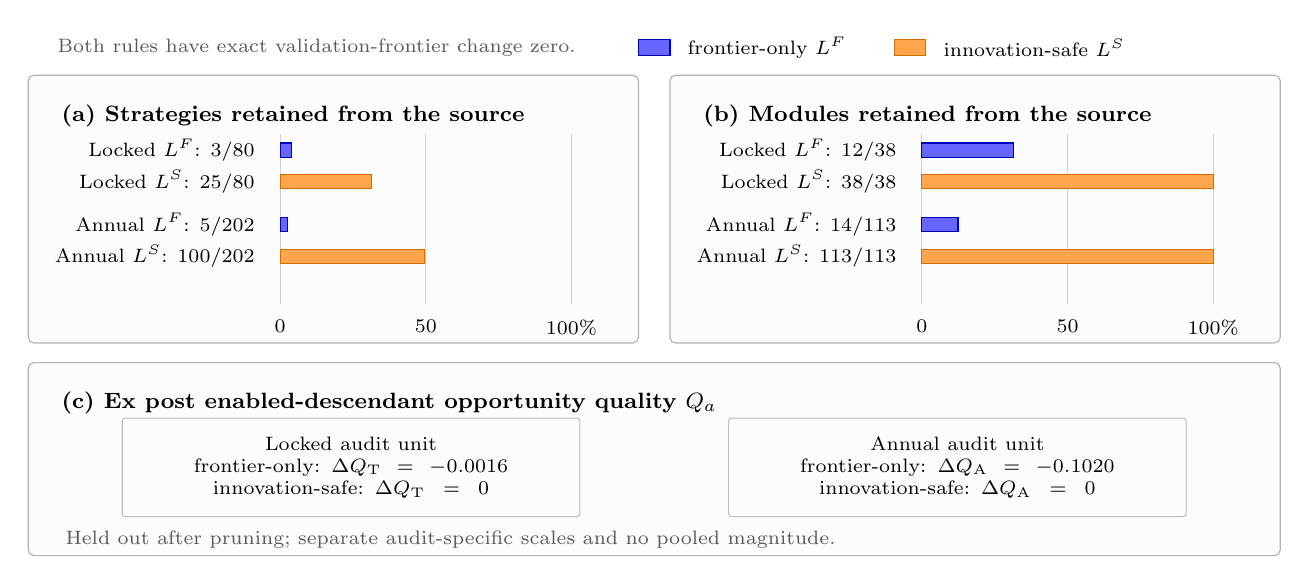
\begin{tikzpicture}[x=1cm,y=1cm,font=\scriptsize]
  \tikzset{
    panel/.style={draw=black!30,rounded corners=2pt,fill=black!1},
    frontier/.style={draw=blue!72!black,fill=blue!60},
    safe/.style={draw=orange!85!black,fill=orange!70},
    title/.style={font=\bfseries\footnotesize,anchor=north west},
    note/.style={font=\scriptsize,anchor=west,text=black!65},
    card/.style={draw=black!25,rounded corners=1pt,align=center,inner sep=3pt}
  }

  % Shared legend and exact zero-frontier-change qualification.
  \draw[frontier] (7.75,6.35) rectangle (8.15,6.55);
  \node[anchor=west] at (8.25,6.45) {frontier-only \(L^F\)};
  \draw[safe] (11.00,6.35) rectangle (11.40,6.55);
  \node[anchor=west] at (11.50,6.45) {innovation-safe \(L^S\)};
  \node[anchor=west,text=black!65] at (0.25,6.45)
    {Both rules have exact validation-frontier change zero.};

  % (a) Fraction of source strategies retained.
  \draw[panel] (0,2.70) rectangle (7.75,6.10);
  \node[title] at (0.30,5.85) {(a) Strategies retained from the source};
  \foreach \x/\label in {3.2/0,5.05/50,6.9/100\%} {
    \draw[black!18] (\x,3.20) -- (\x,5.35);
    \node[anchor=north] at (\x,3.12) {\label};
  }
  \node[anchor=east] at (3.00,5.15) {Locked \(L^F\): 3/80};
  \draw[frontier] (3.2,5.06) rectangle (3.33875,5.24);
  \node[anchor=east] at (3.00,4.75) {Locked \(L^S\): 25/80};
  \draw[safe] (3.2,4.66) rectangle (4.35625,4.84);
  \node[anchor=east] at (3.00,4.20) {Annual \(L^F\): 5/202};
  \draw[frontier] (3.2,4.11) rectangle (3.291584,4.29);
  \node[anchor=east] at (3.00,3.80) {Annual \(L^S\): 100/202};
  \draw[safe] (3.2,3.71) rectangle (5.031683,3.89);

  % (b) Fraction of source modules retained.
  \draw[panel] (8.15,2.70) rectangle (15.90,6.10);
  \node[title] at (8.45,5.85) {(b) Modules retained from the source};
  \foreach \x/\label in {11.35/0,13.2/50,15.05/100\%} {
    \draw[black!18] (\x,3.20) -- (\x,5.35);
    \node[anchor=north] at (\x,3.12) {\label};
  }
  \node[anchor=east] at (11.15,5.15) {Locked \(L^F\): 12/38};
  \draw[frontier] (11.35,5.06) rectangle (12.518421,5.24);
  \node[anchor=east] at (11.15,4.75) {Locked \(L^S\): 38/38};
  \draw[safe] (11.35,4.66) rectangle (15.05,4.84);
  \node[anchor=east] at (11.15,4.20) {Annual \(L^F\): 14/113};
  \draw[frontier] (11.35,4.11) rectangle (11.808407,4.29);
  \node[anchor=east] at (11.15,3.80) {Annual \(L^S\): 113/113};
  \draw[safe] (11.35,3.71) rectangle (15.05,3.89);

  % (c) Ex post enabled-descendant quality; audit units are not pooled.
  \draw[panel] (0,0) rectangle (15.90,2.45);
  \node[title] at (0.30,2.20) {(c) Ex post enabled-descendant opportunity quality \(Q_a\)};
  \node[card,text width=5.60cm,minimum height=1.25cm] at (4.10,1.12)
    {Locked audit unit\\frontier-only: \(\Delta Q_{\mathrm T}=-0.0016\)\\
     innovation-safe: \(\Delta Q_{\mathrm T}=0\)};
  \node[card,text width=5.60cm,minimum height=1.25cm] at (11.80,1.12)
    {Annual audit unit\\frontier-only: \(\Delta Q_{\mathrm A}=-0.1020\)\\
     innovation-safe: \(\Delta Q_{\mathrm A}=0\)};
  \node[note] at (0.35,0.20) {Held out after pruning; separate audit-specific scales and no pooled magnitude.};
\end{tikzpicture}
